%
\section{Implementation}
\label{sec:impl}

Our solution is designed using commodity off the shelf (COTS) components.
The open-source implementation\footnote{Available at: \url{https://github.com/synercys/PIRMedic}} includes:

\ca \textbf{Edge Hardware} consisting of -- \ci a PIR sensor~\cite{PIR_sensor_eval}, \cii a bare-metal platform~\viz Arduino Mega Microcontroller Unit (MCU)~\cite{arduino_mega} 
for sensor data capture, and \ciii a Linux-based platform~\viz Raspberry Pi~\cite{rpi3} 
for executing the fault detection and diagnosis algorithm, \sol. The specifications of hardware used can be seen in {\bfseries Table~\ref{tab:pir_platform}}.%

The Arduino MCU polls the sensor hardware signals (\ie \cout and \aout) periodically over a GPIO interface. We poll the PIR sensors at a frequency $\geq$ 20 Hz due to the \textit{Nyquist criterion} as the human motion information in the PIR sensor is between 0 -- 10 Hz. %
Note that using a bare-metal platform allows us to capture \aout samples at a constant rate. %
The Raspberry Pi platform performs the fault detection and analysis for the data captured at the Arduino MCU.
The Raspberry Pi and Arduino are connected via a Micro-USB cable and the data captured at the Arduino MCU is serially transferred to the Raspberry Pi for analysis, as shown in {\bfseries Fig.~\ref{fig:eval_platform}}.%

\begin{figure}
	\begin{minipage}[t][4 cm][c]{0.28\textwidth}
		\centering
		%\noindent
		%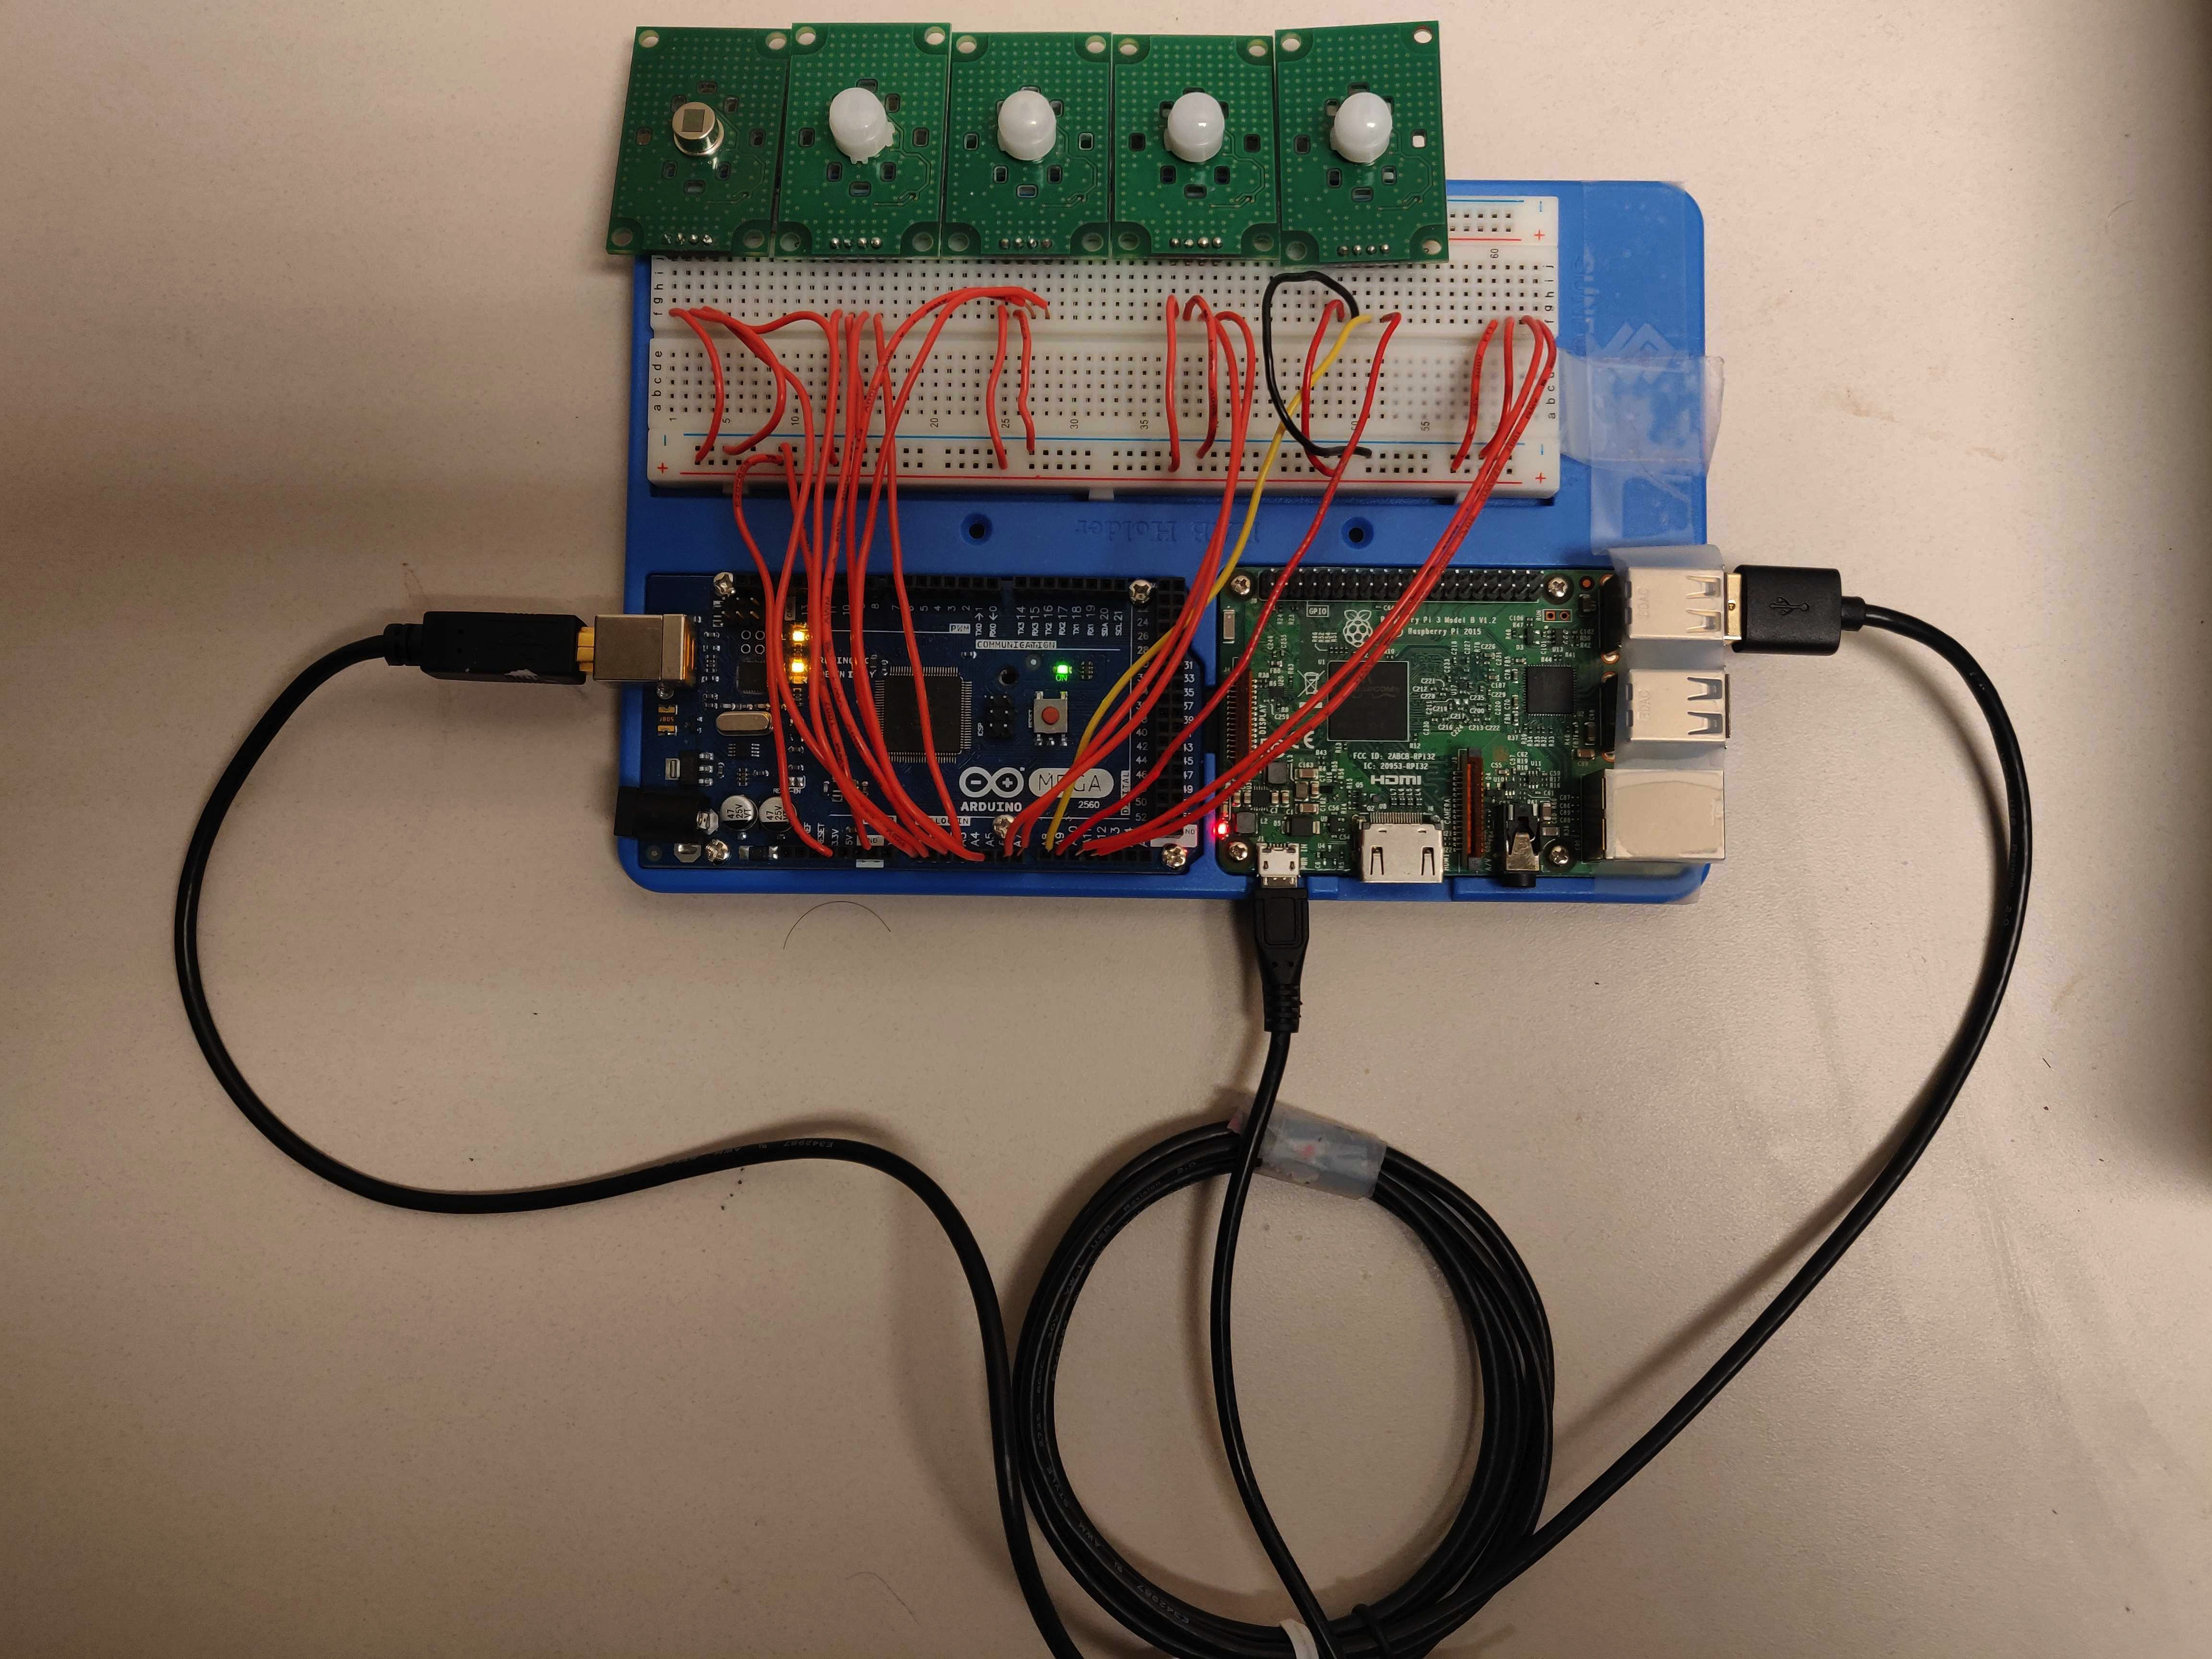
\includegraphics[width=0.9\textwidth, height=1.1in]{figures/platform/eval_platform.jpg}
		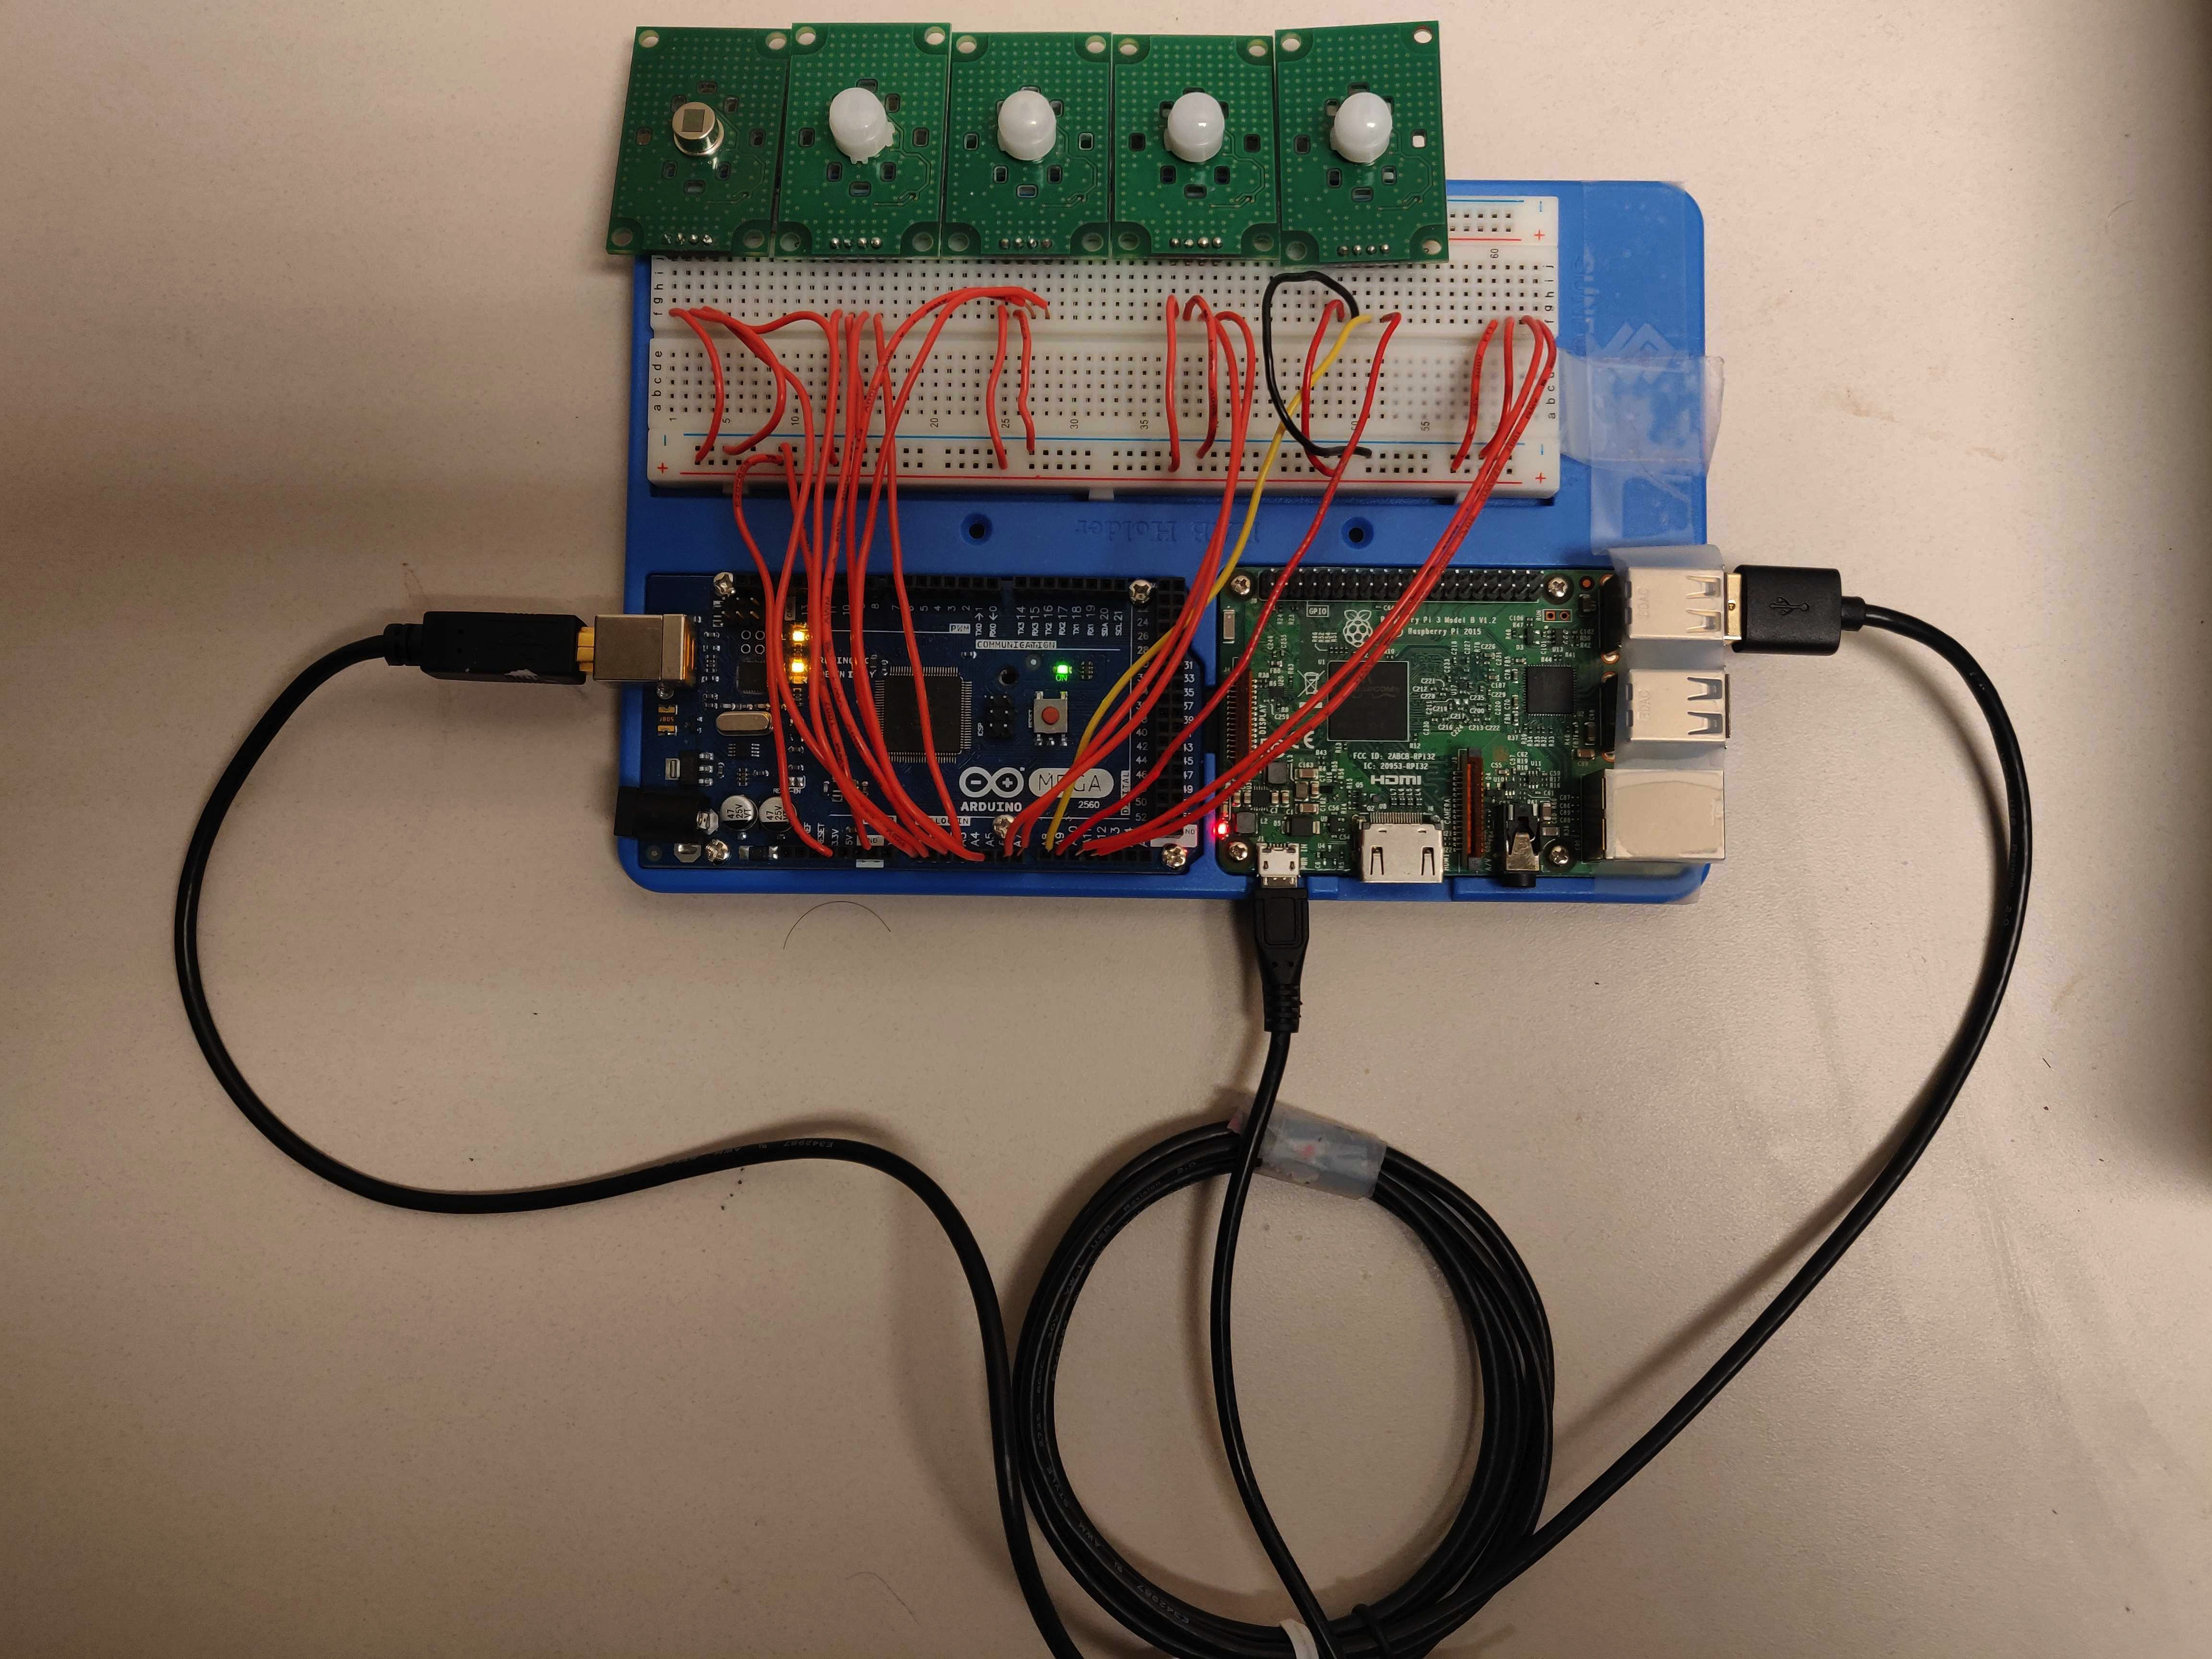
\includegraphics[scale=0.022]{figures/platform/eval_platform.jpg}
		\captionof{figure}{Evaluation Platform showing PIR sensor connected to Raspberry Pi and Arduino.}
		\label{fig:eval_platform}
	\end{minipage}
	\hfill
	\begin{minipage}[t][4cm][c]{0.70\textwidth}
		\centering
		\vspace*{\fill}
		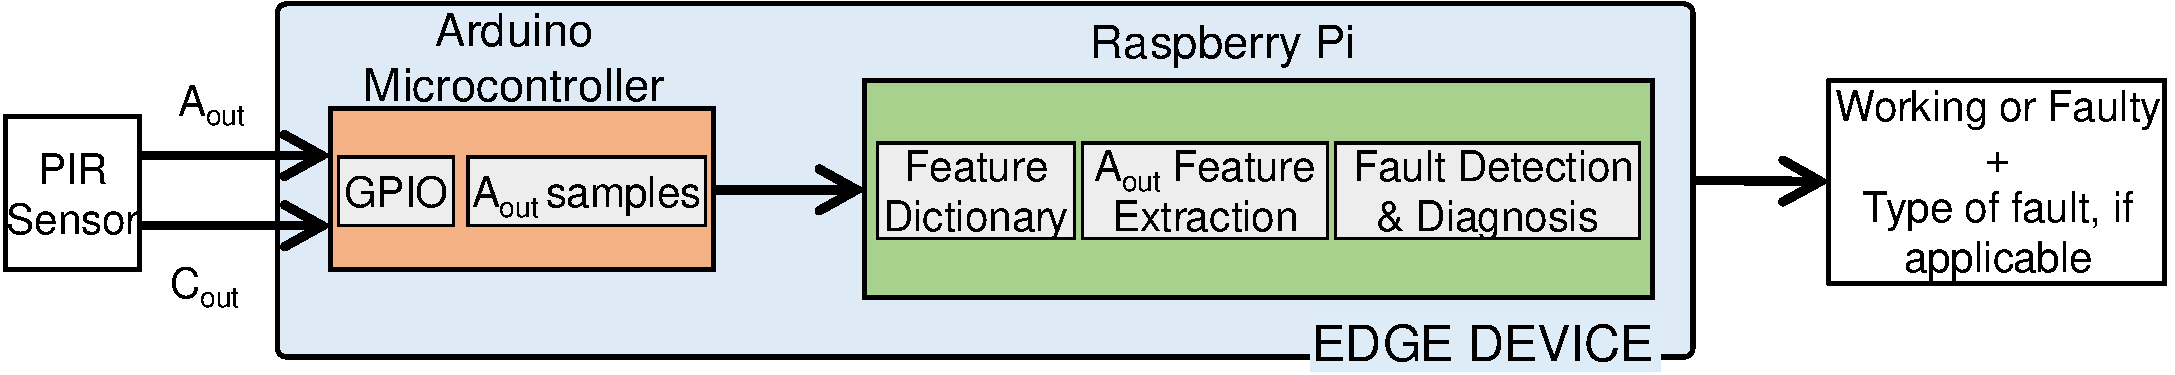
\includegraphics[width=\textwidth]{figures/platform/sensys_workflow.pdf}
		\vspace*{\fill}
		\caption{\sol workflow. The PIR sensor is connected to an Arduino microcontroller via a GPIO interface. An ADC onboard the microcontroller converts \aout and \cout values into discrete samples, that are sent to a Raspberry Pi for fault detection and diagnosis.}
		\label{fig:system_workflow}
	\end{minipage}%
\end{figure}%
%

\cb \textbf{Edge Implementation} We used standard python libraries such as \texttt{tsfresh}~\cite{tsfresh2018code,christ2016distributed} for computing features such as FFT and other statistical features as a part pf feature extraction, \texttt{numpy} for data preprocessing and \texttt{xgboost}~\cite{shap_implementation} for implementing the machine learning classifiers. %
The end-to-end workflow of our solution is illustrated in {\bfseries Fig.~\ref{fig:system_workflow}}.

\subsection{Parameters of \sol}
\label{subsec:prac}

\ci \textbf{Size of Window}: The collected \aout waveform is split into equal-size sample windows over which features are calculated. We observed that using a window too small (\eg 128) does not allow us to capture sufficient features for a failure type and could lead to a large number of false alarms. Also, too large of a window size (\eg 8192) leads to an overlap in the features of multiple failure classes leading to a loss of accuracy. The variation of model accuracy as a function of window size is shown in {\bfseries Fig.~\ref{fig:accuracy_vs_window_size}}. We chose a window size of 1024 samples as it gave us a good trade-off between time to capture a window (approx. 50 seconds) and accuracy (> 98\%).

\begin{figure}%{lr}{0.5\textwidth}
	\centering
	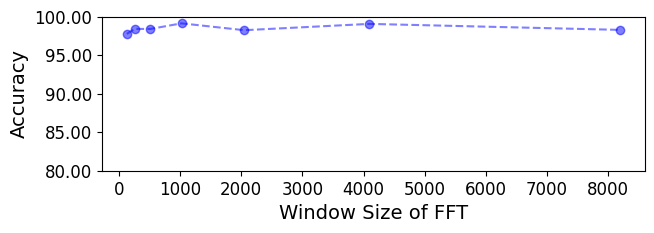
\includegraphics[width=0.48\textwidth]{figures/classification/accuracy_vs_window_size.png}
	\caption{Model Accuracy for different window sizes. We choose 1024 as the default window size.}
	\label{fig:accuracy_vs_window_size}
\end{figure}

\cii \textbf{Benjamini-Hochberg (B-H) Feature Selection} While there are more than 300 features that can be derived for time series analysis of \aout, B-H feature selection process (derived from parameterized hypothesis testing)~\cite{benjamini1995controlling,christ2018time} prunes this to a lower number of features that can sufficiently capture the physics of the system. We observed that using more than 10 features did not contribute to a significant increase in accuracy (beyond 98\%) and can, in practice, lead to lower performance due to overfitting as described in \S\ref{subsec:bh}.%

\ciii \textbf{Classifier Model}: We used a Random Forest classifier~\cite{polikar2012ensemble, breiman2001random} owing to the capability to classify data based on ``entropy'' or the information gain.  %
Random Forest uses an ensemble of trees and has been shown to give high predictive accuracy and control over-fitting in practice, both of which are issues with decision trees. Additionally, Random Forests are amenable to interpretation by techniques such as Shapley TreeExplainer~\cite{lundberg2020local2global} that explains the features influencing prediction. \textit{Finally, we note that \aout is compatible with any classification algorithm.}

